\chapter{Data Service: Central Data Store}
\label{chap:data-service}

The previous chapter introduced the \textbf{Petri Net Elements}---the individual building blocks (places, transitions, arcs) of our models. This chapter focuses on the \textbf{Data Service}, which acts as the central repository for all these elements and ensures the entire application stays synchronized.

\section{Problem Statement}
\label{sec:data-problem}

Consider what happens when you \textbf{add a new Place} to your Petri net:

\begin{enumerate}
    \item You drag a ``Place'' icon onto the canvas
    \item The application creates a new \texttt{Place} object in memory
    \item This new place must be \textbf{stored} somewhere accessible
    \item The \textbf{drawing component} must know about it to render it
    \item The \textbf{save function} must include it when exporting
    \item The \textbf{simulation engine} must consider it when calculating enabled transitions
\end{enumerate}

Without a central data store, every component would maintain its own list of elements. If one component adds a place, how do the others know? If one deletes an arc, how do the others update? This would lead to:

\begin{itemize}
    \item \textbf{Inconsistent state}: Different components showing different data
    \item \textbf{Complex synchronization}: Manual coordination between components
    \item \textbf{Bug-prone code}: Easy to forget updating one of many lists
\end{itemize}

The \texttt{DataService} solves this by being the \textbf{single source of truth} for all Petri net data.

\section{Conceptual Overview}
\label{sec:data-concept}

Think of the \texttt{DataService} as the application's \textbf{central brain} or \textbf{shared whiteboard}. It maintains:

\begin{itemize}
    \item \textbf{All Places}: Their tokens, positions, IDs, and labels
    \item \textbf{All Transitions}: Their positions, IDs, labels, and connected arcs
    \item \textbf{All Arcs}: Source/target nodes, weights, and anchor points
    \item \textbf{All Actions}: Unique labels used by transitions
\end{itemize}

When anything changes, the \texttt{DataService}:
\begin{enumerate}
    \item Updates its internal records
    \item \textbf{Broadcasts} the change to all interested components
\end{enumerate}

This ensures every part of the application sees the same, up-to-date data.

\section{Implementation}
\label{sec:data-implementation}

\begin{lstlisting}[language=TypeScript, caption={DataService core implementation (src/app/tr-services/data.service.ts)}]
import { Injectable } from '@angular/core';
import { Subject, Observable } from 'rxjs';
import { Arc } from '../tr-classes/petri-net/arc';
import { Place } from '../tr-classes/petri-net/place';
import { Transition } from '../tr-classes/petri-net/transition';

/**
 * Payload emitted when data changes.
 * fitContent: if true, the UI should re-center the view on the net.
 */
interface DataChangedPayload {
    fitContent: boolean;
}

@Injectable({
    providedIn: 'root', // Singleton: one instance for entire application
})
export class DataService {
    // =========================================================================
    // PRIVATE DATA STORAGE
    // =========================================================================
    
    /** All places in the current Petri net */
    private _places: Place[] = [];
    
    /** All transitions in the current Petri net */
    private _transitions: Transition[] = [];
    
    /** All arcs connecting places and transitions */
    private _arcs: Arc[] = [];
    
    /** Unique action labels used by transitions */
    private _actions: string[] = [];

    // =========================================================================
    // CHANGE NOTIFICATION
    // =========================================================================
    
    /**
     * Subject for broadcasting data changes.
     * Components subscribe to be notified when the Petri net is modified.
     */
    private dataChangedSubject = new Subject<DataChangedPayload>();
    
    /** Public observable for subscribing to data changes */
    public dataChanged$: Observable<DataChangedPayload> = 
        this.dataChangedSubject.asObservable();

    // =========================================================================
    // GETTERS: Read current data
    // =========================================================================
    
    getPlaces(): Place[] { return this._places; }
    getTransitions(): Transition[] { return this._transitions; }
    getArcs(): Arc[] { return this._arcs; }
    getActions(): string[] { return this._actions; }

    // =========================================================================
    // SETTERS: Replace entire collections (used when loading files)
    // =========================================================================
    
    set places(value: Place[]) { this._places = value; }
    set transitions(value: Transition[]) { this._transitions = value; }
    set arcs(value: Arc[]) { this._arcs = value; }
    set actions(value: string[]) { this._actions = value; }

    // =========================================================================
    // MODIFICATION METHODS
    // =========================================================================

    /**
     * Add a new place to the Petri net.
     */
    addPlace(place: Place): void {
        this._places.push(place);
        this.triggerDataChanged();
    }

    /**
     * Remove a place and all its connected arcs.
     */
    removePlace(deletablePlace: Place): void {
        // First, remove all arcs connected to this place
        const connectedArcs = this._arcs.filter(
            arc => arc.from === deletablePlace || arc.to === deletablePlace
        );
        connectedArcs.forEach(arc => this.removeArc(arc));

        // Then remove the place itself
        this._places = this._places.filter(place => place !== deletablePlace);
        
        this.triggerDataChanged();
    }

    /**
     * Add a new transition to the Petri net.
     */
    addTransition(transition: Transition): void {
        this._transitions.push(transition);
        this.triggerDataChanged();
    }

    /**
     * Remove a transition and all its connected arcs.
     */
    removeTransition(deletableTransition: Transition): void {
        // Remove connected arcs
        const connectedArcs = this._arcs.filter(
            arc => arc.from === deletableTransition || arc.to === deletableTransition
        );
        connectedArcs.forEach(arc => this.removeArc(arc));

        // Remove the transition
        this._transitions = this._transitions.filter(t => t !== deletableTransition);
        
        this.triggerDataChanged();
    }

    /**
     * Connect two nodes with a new arc.
     * Validates that the connection follows Petri net rules:
     * - Place -> Transition (input arc)
     * - Transition -> Place (output arc)
     */
    connectNodes(from: Node, to: Node): Arc | null {
        // Validate: cannot connect Place to Place or Transition to Transition
        if (from instanceof Place && to instanceof Place) {
            console.error('Cannot connect Place to Place');
            return null;
        }
        if (from instanceof Transition && to instanceof Transition) {
            console.error('Cannot connect Transition to Transition');
            return null;
        }

        const arc = new Arc(from, to, 1);
        this._arcs.push(arc);

        // Register arc with the transition
        if (from instanceof Place && to instanceof Transition) {
            to.appendPreArc(arc);  // Input arc
        } else if (from instanceof Transition && to instanceof Place) {
            from.appendPostArc(arc);  // Output arc
        }

        this.triggerDataChanged();
        return arc;
    }

    /**
     * Remove an arc from the Petri net.
     */
    removeArc(arc: Arc): void {
        this._arcs = this._arcs.filter(a => a !== arc);
        
        // Also remove from transition's arc lists
        if (arc.to instanceof Transition) {
            arc.to.preArcs = arc.to.preArcs.filter(a => a !== arc);
        }
        if (arc.from instanceof Transition) {
            arc.from.postArcs = arc.from.postArcs.filter(a => a !== arc);
        }
    }

    // =========================================================================
    // UTILITY METHODS
    // =========================================================================

    /**
     * Find a place by its ID.
     */
    getPlaceById(id: string): Place | undefined {
        return this._places.find(p => p.id === id);
    }

    /**
     * Find a transition by its ID.
     */
    getTransitionById(id: string): Transition | undefined {
        return this._transitions.find(t => t.id === id);
    }

    /**
     * Check if the Petri net is empty.
     */
    isEmpty(): boolean {
        return this._places.length === 0 && this._transitions.length === 0;
    }

    /**
     * Clear all data (reset to empty net).
     */
    clearAll(): void {
        this._places = [];
        this._transitions = [];
        this._arcs = [];
        this._actions = [];
        this.triggerDataChanged(true);
    }

    // =========================================================================
    // CHANGE NOTIFICATION
    // =========================================================================

    /**
     * Broadcast that data has changed.
     * All subscribed components will be notified.
     * 
     * @param fitContent If true, UI should re-center the view
     */
    public triggerDataChanged(fitContent: boolean = false): void {
        console.log('[DataService] Data changed, fitContent:', fitContent);
        this.dataChangedSubject.next({ fitContent });
    }
}
\end{lstlisting}

\section{Key Concepts}
\label{sec:data-concepts}

\subsection{Singleton Pattern}

The \texttt{@Injectable(\{providedIn: 'root'\})} decorator ensures only \textbf{one instance} of \texttt{DataService} exists. All components access the same instance, guaranteeing they work with the same data.

\subsection{Subject vs. BehaviorSubject}

Unlike the \texttt{UiService} which uses \texttt{BehaviorSubject} (remembers the last value), the \texttt{DataService} uses a plain \texttt{Subject}:

\begin{itemize}
    \item \textbf{Subject}: Only emits to current subscribers; new subscribers don't receive past events
    \item \textbf{Why?} Components don't need the ``last change event''---they need the \textit{current data}, which they get via \texttt{getPlaces()}, \texttt{getTransitions()}, etc.
\end{itemize}

\subsection{Cascading Deletes}

When removing a place or transition, all connected arcs are automatically removed:

\begin{lstlisting}[language=TypeScript, caption={Cascading delete pattern}]
removePlace(deletablePlace: Place): void {
    // 1. Find connected arcs
    const connectedArcs = this._arcs.filter(
        arc => arc.from === deletablePlace || arc.to === deletablePlace
    );
    
    // 2. Remove each connected arc
    connectedArcs.forEach(arc => this.removeArc(arc));
    
    // 3. Remove the place itself
    this._places = this._places.filter(place => place !== deletablePlace);
    
    // 4. Notify subscribers
    this.triggerDataChanged();
}
\end{lstlisting}

\section{Usage Patterns}
\label{sec:data-usage}

\subsection{Adding Elements}

\begin{lstlisting}[language=TypeScript, caption={Adding a place via DataService}]
import { Component } from '@angular/core';
import { DataService } from 'src/app/tr-services/data.service';
import { Place } from 'src/app/tr-classes/petri-net/place';
import { Point } from 'src/app/tr-classes/petri-net/point';

@Component({ /* ... */ })
export class PetriNetComponent {
    constructor(private dataService: DataService) {}

    /**
     * Called when user clicks on canvas with "Add Place" tool selected.
     */
    onCanvasClick(x: number, y: number): void {
        // Generate unique ID
        const newId = `p${this.dataService.getPlaces().length + 1}`;
        
        // Create the place object
        const newPlace = new Place(0, new Point(x, y), newId);
        
        // Add to DataService (automatically notifies subscribers)
        this.dataService.addPlace(newPlace);
    }
}
\end{lstlisting}

\subsection{Subscribing to Changes}

\begin{lstlisting}[language=TypeScript, caption={Subscribing to data changes}]
import { Component, OnInit, OnDestroy } from '@angular/core';
import { Subscription } from 'rxjs';
import { DataService } from 'src/app/tr-services/data.service';

@Component({ /* ... */ })
export class DrawingCanvasComponent implements OnInit, OnDestroy {
    private dataSubscription: Subscription;

    constructor(private dataService: DataService) {}

    ngOnInit(): void {
        // Subscribe to data changes
        this.dataSubscription = this.dataService.dataChanged$.subscribe(payload => {
            console.log('Data changed! Redrawing...');
            
            // Get latest data
            const places = this.dataService.getPlaces();
            const transitions = this.dataService.getTransitions();
            const arcs = this.dataService.getArcs();
            
            // Redraw the canvas
            this.redraw(places, transitions, arcs);
            
            // Optionally re-center the view
            if (payload.fitContent) {
                this.fitContentToViewport();
            }
        });

        // Initial draw
        this.redraw(
            this.dataService.getPlaces(),
            this.dataService.getTransitions(),
            this.dataService.getArcs()
        );
    }

    ngOnDestroy(): void {
        this.dataSubscription?.unsubscribe();
    }

    private redraw(places: Place[], transitions: Transition[], arcs: Arc[]): void {
        // Clear and redraw SVG elements...
    }
}
\end{lstlisting}

\section{Data Flow Visualization}
\label{sec:data-flow}

\begin{figure}[htb]
    \centering
    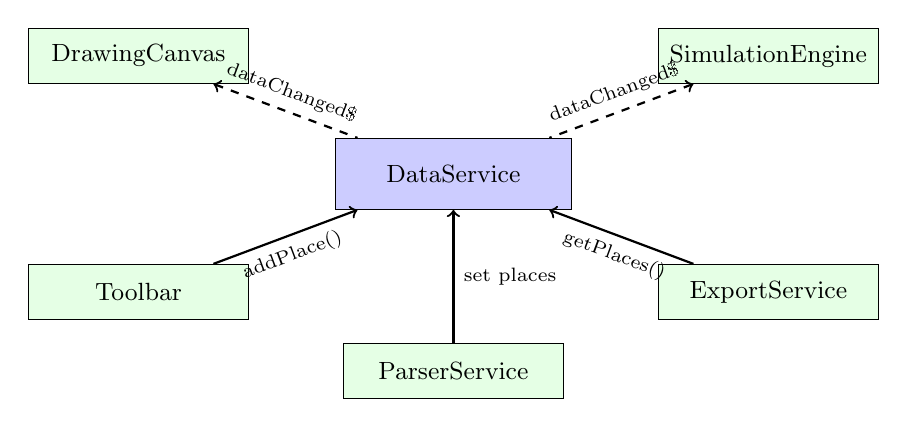
\begin{tikzpicture}[
        node distance=1.2cm,
        component/.style={rectangle, draw, fill=green!10, minimum width=2.8cm, minimum height=0.7cm, font=\small},
        service/.style={rectangle, draw, fill=blue!20, minimum width=3cm, minimum height=0.9cm, font=\small},
    ]
        % Central service
        \node[service] (ds) at (0,0) {DataService};
        
        % Components around it
        \node[component] (canvas) at (-4, 1.5) {DrawingCanvas};
        \node[component] (toolbar) at (-4, -1.5) {Toolbar};
        \node[component] (sim) at (4, 1.5) {SimulationEngine};
        \node[component] (export) at (4, -1.5) {ExportService};
        \node[component] (parser) at (0, -2.5) {ParserService};
        
        % Arrows
        \draw[->, thick] (toolbar) -- node[below, sloped, font=\scriptsize] {addPlace()} (ds);
        \draw[->, thick] (parser) -- node[right, font=\scriptsize] {set places} (ds);
        \draw[<-, thick, dashed] (canvas) -- node[above, sloped, font=\scriptsize] {dataChanged\$} (ds);
        \draw[<-, thick, dashed] (sim) -- node[above, sloped, font=\scriptsize] {dataChanged\$} (ds);
        \draw[->, thick] (export) -- node[below, sloped, font=\scriptsize] {getPlaces()} (ds);
        
    \end{tikzpicture}
    \caption{DataService as central hub for Petri net data}
    \label{fig:data-service-hub}
\end{figure}

The diagram shows:
\begin{itemize}
    \item \textbf{Solid arrows}: Components that \textit{modify} data (Toolbar adds elements, ParserService loads files)
    \item \textbf{Dashed arrows}: Components that \textit{subscribe} to changes (Canvas redraws, SimulationEngine recalculates)
    \item \textbf{Query arrows}: Components that \textit{read} data on demand (ExportService for saving)
\end{itemize}

\section{Interaction with Other Services}
\label{sec:data-interactions}

The \texttt{DataService} is used by nearly every other service:

\begin{table}[htb]
    \centering
    \begin{tabular}{ll}
        \toprule
        \textbf{Service} & \textbf{Interaction} \\
        \midrule
        \texttt{ParserService} & Loads data from JSON/PNML files \\
        \texttt{PnmlService} & Imports/exports PNML format \\
        \texttt{ExportJsonDataService} & Exports to custom JSON format \\
        \texttt{LayoutSugiyamaService} & Modifies element positions \\
        \texttt{ZoomService} & Reads element positions for bounds calculation \\
        \texttt{SimulationService} & Reads transitions for firing sequence \\
        \bottomrule
    \end{tabular}
    \caption{Services that interact with DataService}
    \label{tab:data-service-interactions}
\end{table}

\section{Summary}
\label{sec:data-summary}

The \texttt{DataService} is the application's \textbf{single source of truth} for Petri net data:

\begin{itemize}
    \item \textbf{Stores} all places, transitions, arcs, and actions
    \item \textbf{Provides} getter methods for reading current state
    \item \textbf{Offers} modification methods with automatic cascading (e.g., deleting connected arcs)
    \item \textbf{Broadcasts} changes via \texttt{dataChanged\$} observable
    \item \textbf{Enables} decoupled architecture where components don't directly communicate
\end{itemize}

With the core data model and storage understood, the next chapter explores how users interact with the canvas through \textbf{Zoom and Pan} functionality.
